\documentclass[a4paper,12pt]{article}
\addtolength{\oddsidemargin}{-1.cm}
\addtolength{\textwidth}{2cm}
\addtolength{\topmargin}{-2cm}
\addtolength{\textheight}{3.5cm}
\newcommand{\HRule}{\rule{\linewidth}{0.5mm}}
\makeindex

\usepackage{longtable}
\usepackage[pdftex]{graphicx}
\usepackage{makeidx}
\usepackage{hyperref}
\usepackage{verbatim}
\hypersetup{
    colorlinks=true,
    linkcolor=blue,
    filecolor=magenta,      
    urlcolor=cyan,
}


% define the title
\author{IMAPKD}
\title{ Project Tender}
\begin{document}
\setlength{\parskip}{6pt}

% generates the title
\begin{titlepage}

\begin{center}
% Upper part of the page       

\includegraphics[width=1\textwidth]{./University_of_Pretoria_Logo.PNG}\\[0.4cm]    
\textsc{\Large Project Tender}\\[0.5cm]
% Title
\rule{15cm}{0.5pt}

{ \huge \textsc Project: VizARD(Augmented Reality Data Visualization) }\\[0.4cm]\
{ \huge \textsc Client: EPI-USE Labs  }

\rule{15cm}{0.4pt}
\\[0.5cm]
{ \huge \textsc Team: IMPAKD  }\\[0.1cm]\

\textsc{\Large\underline{Team Members}}\\[0.5cm]

{\Large Diana {Obo}} \\[0.3cm]

{\Large Kudzai {Muranga}} \\[0.3cm]

{\Large Priscilla {Madigoe}}\\[0.3cm]

{\Large Sandile {Khumalo}}\\[0.5cm]

\textsc{ Department Of Computer Science, University of Pretoria}\\[0.3cm]
\textsc{Date: 2 May 2016}\\[0.3cm]

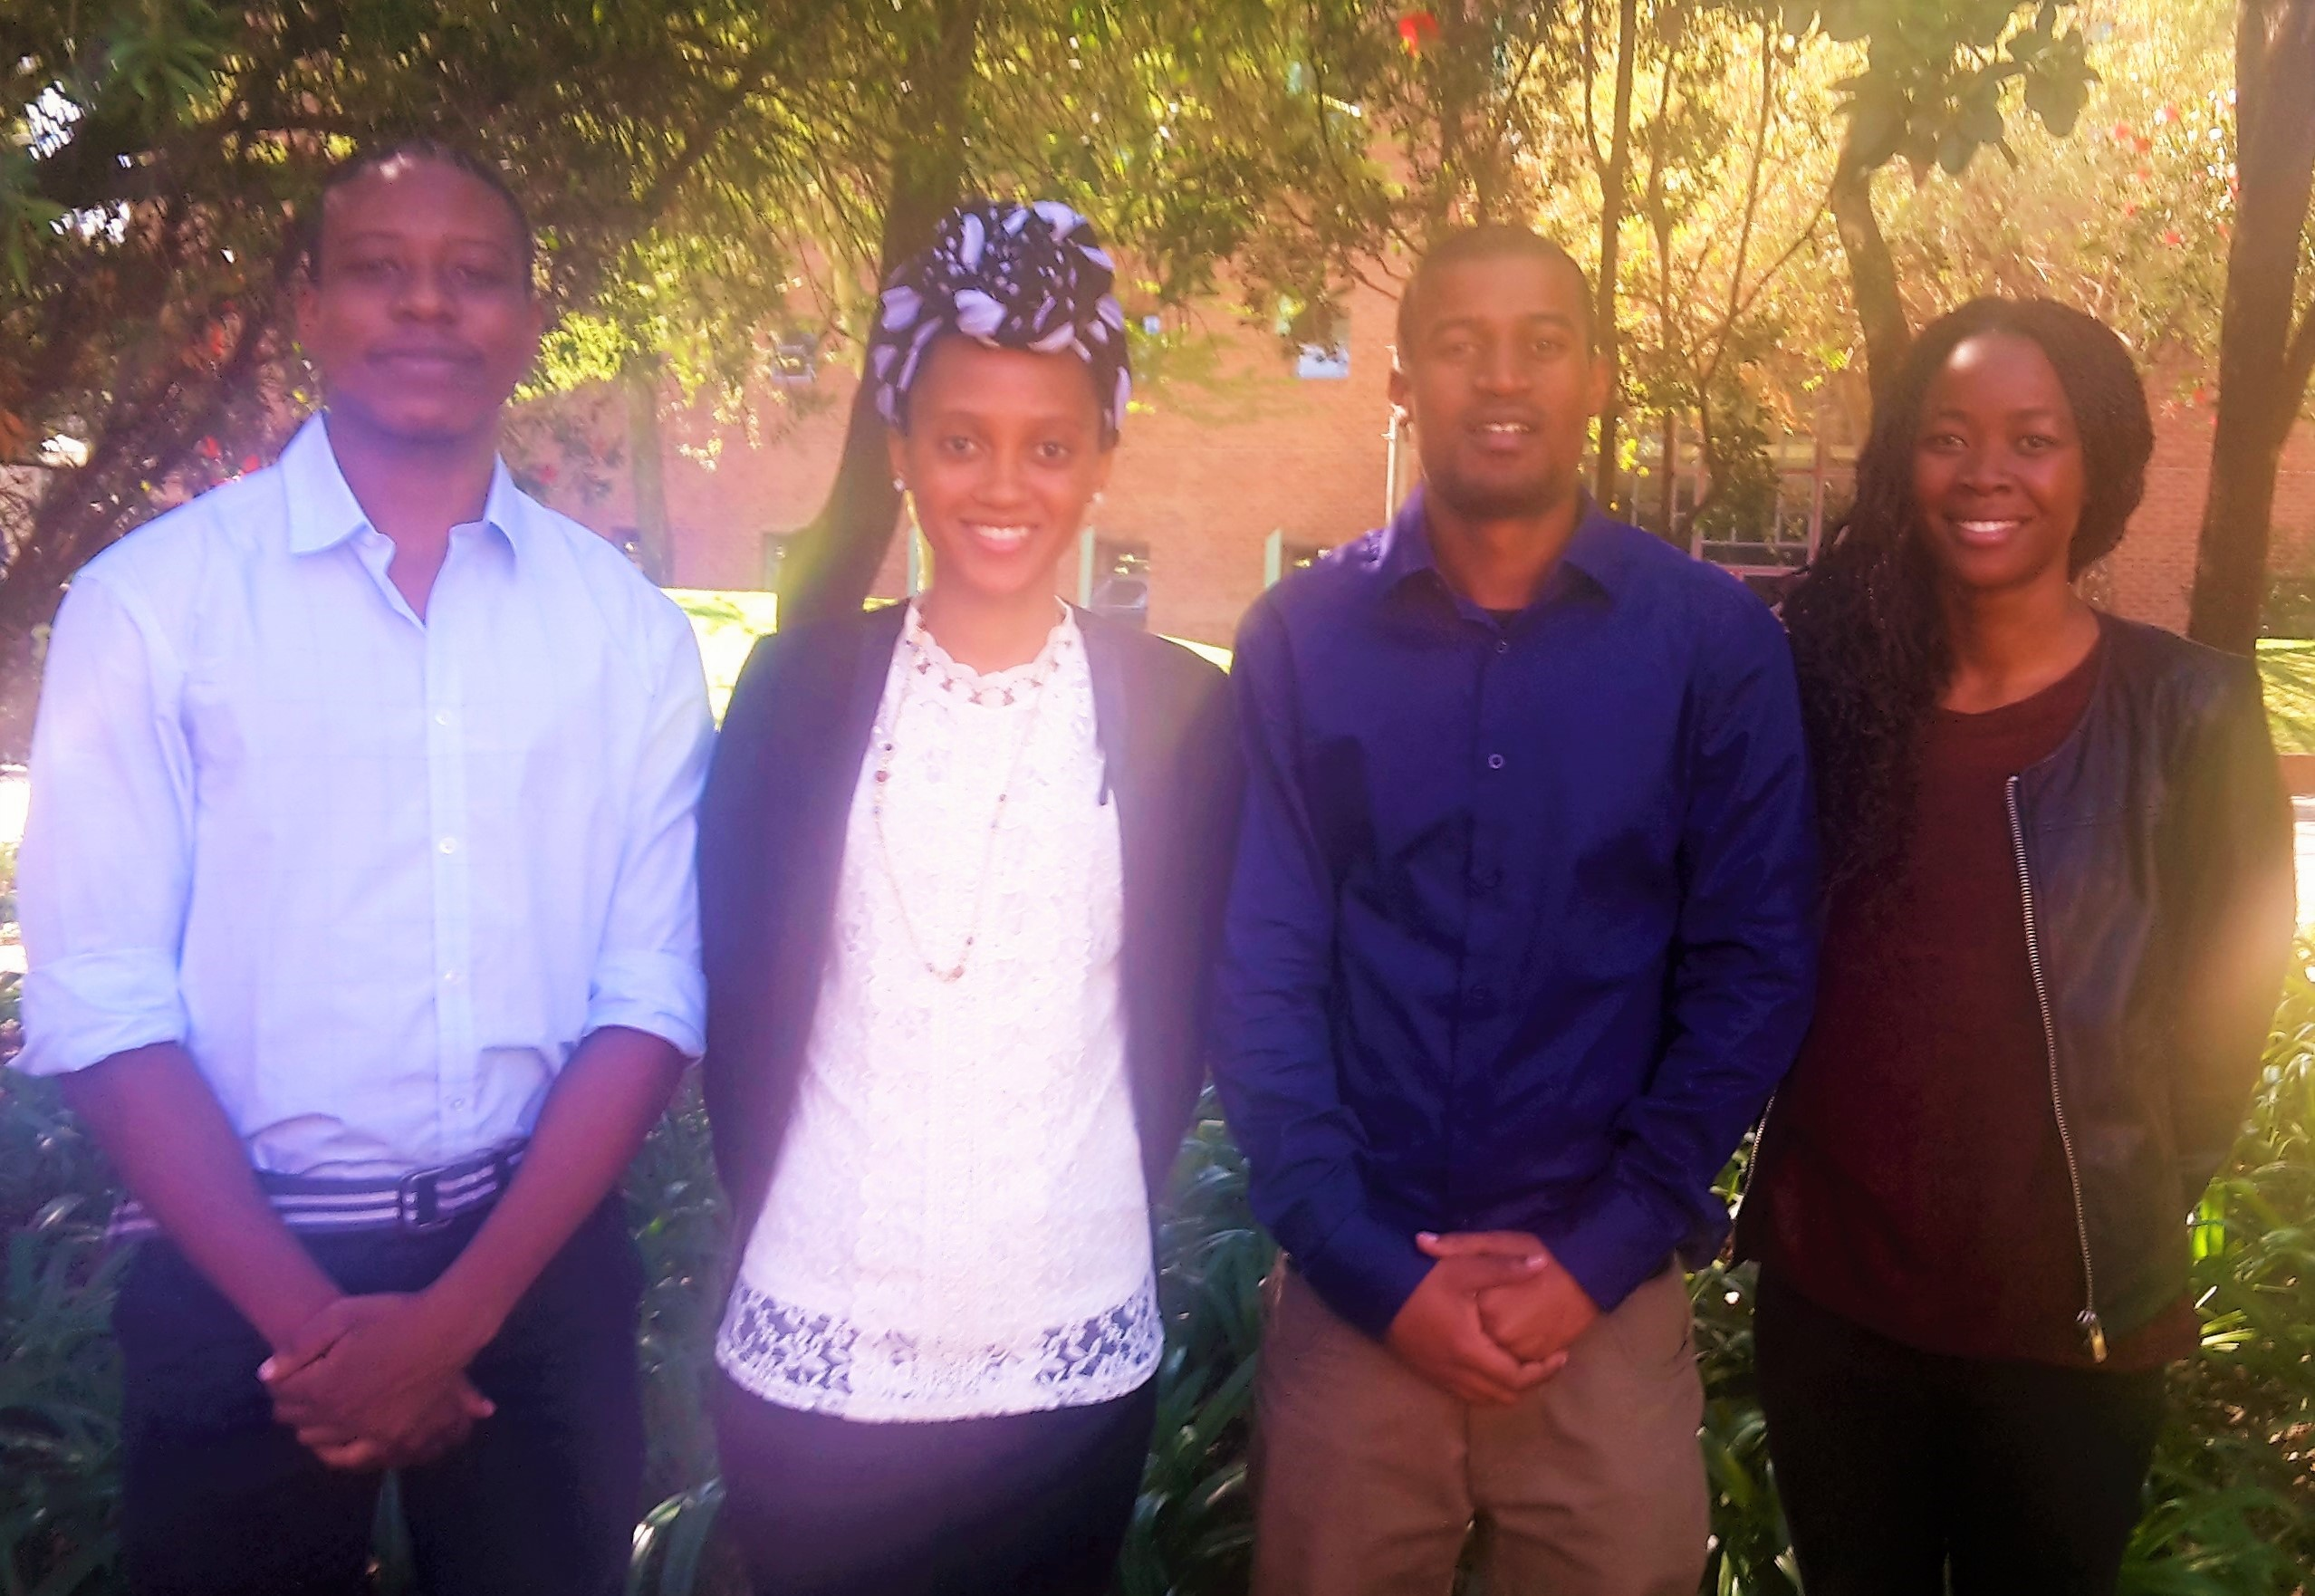
\includegraphics[width=3in]{./IMAPKD.jpg}

\vfill
% Bottom of the page
\end{center}
\end{titlepage}

\newpage
\section{Meet the Team Members}

%Priscilla Madigoe's Section - beginning

\begin{center}
{\Large Priscilla {Madigoe}} \\[0.3cm]
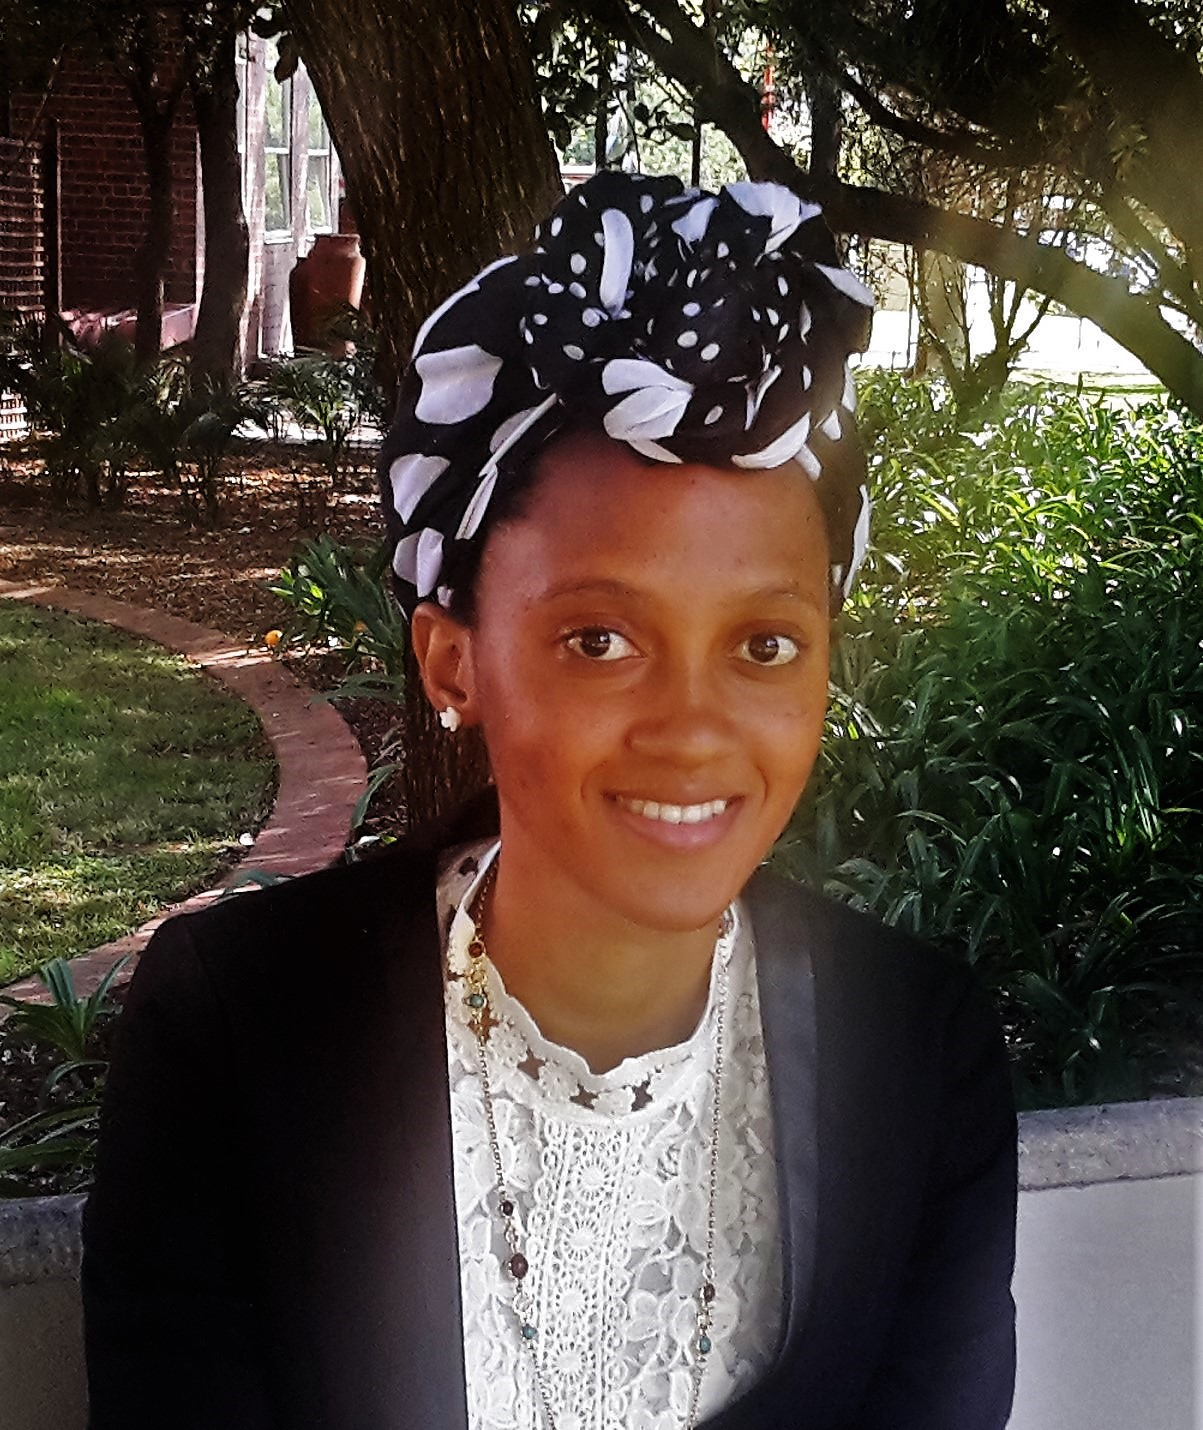
\includegraphics[width= 2in]{P.jpg}\\[0.4cm] 
\end{center}

\begin{itemize}
\item {\large \underline{\textbf{Interests}}}\\[0.2cm]
My interests include Computer Programming, Electronics, Computer Graphics, Robotics, travelling, photography, music, sports and reading novels.
\\
\item {\large \underline{\textbf{Technical Skills}}}

	\begin{itemize}
		\item Computer Programming with sound knowledge of Java, C/C++, MatLab, WebGL and Web-related 					programming languages.
		\item Complex Problem-Solving using scientific and mathematical principles.
		\item System Analysis to determine how a computer software should behave in set conditions.
		\item Quality Control Analysis to evaluate the performance and quality of computer software.
	\end{itemize}
\bigskip
\item {\large \underline{\textbf{Past Experience}}}\\[0.2cm]
The Software Engineering module had a preparatory project called the Mini Project that was created to give students a real-world experience of software development. I took part in the project and I have learnt the process of software development, team work and different technologies used to develop computer software. I have participated in this year's Standard Bank IT Challenge. 
\\
\item {\large \underline{\textbf{Non-Technical Skills}}}\\[0.2cm]
My non-technical skills include critical thinking, reading comprehension, writing, effective listening, social perceptiveness and active learning. 
\\
\item {\large \underline{\textbf{Reason for Interest in the Project}}}\\[0.2cm]
I would like to expand my knowledge on Computer Graphics and Augmented Reality as I am currently enrolled in an elementary Computer Graphics course. This project will help me gain insight on how to apply Computer Graphics for Game Development.

\end{itemize}
%Priscilla Madigoe's Section - end 

\newpage

% Diana Obo's Section - start
\begin{center}
{\Large Diana {Obo}} \\[0.3cm]
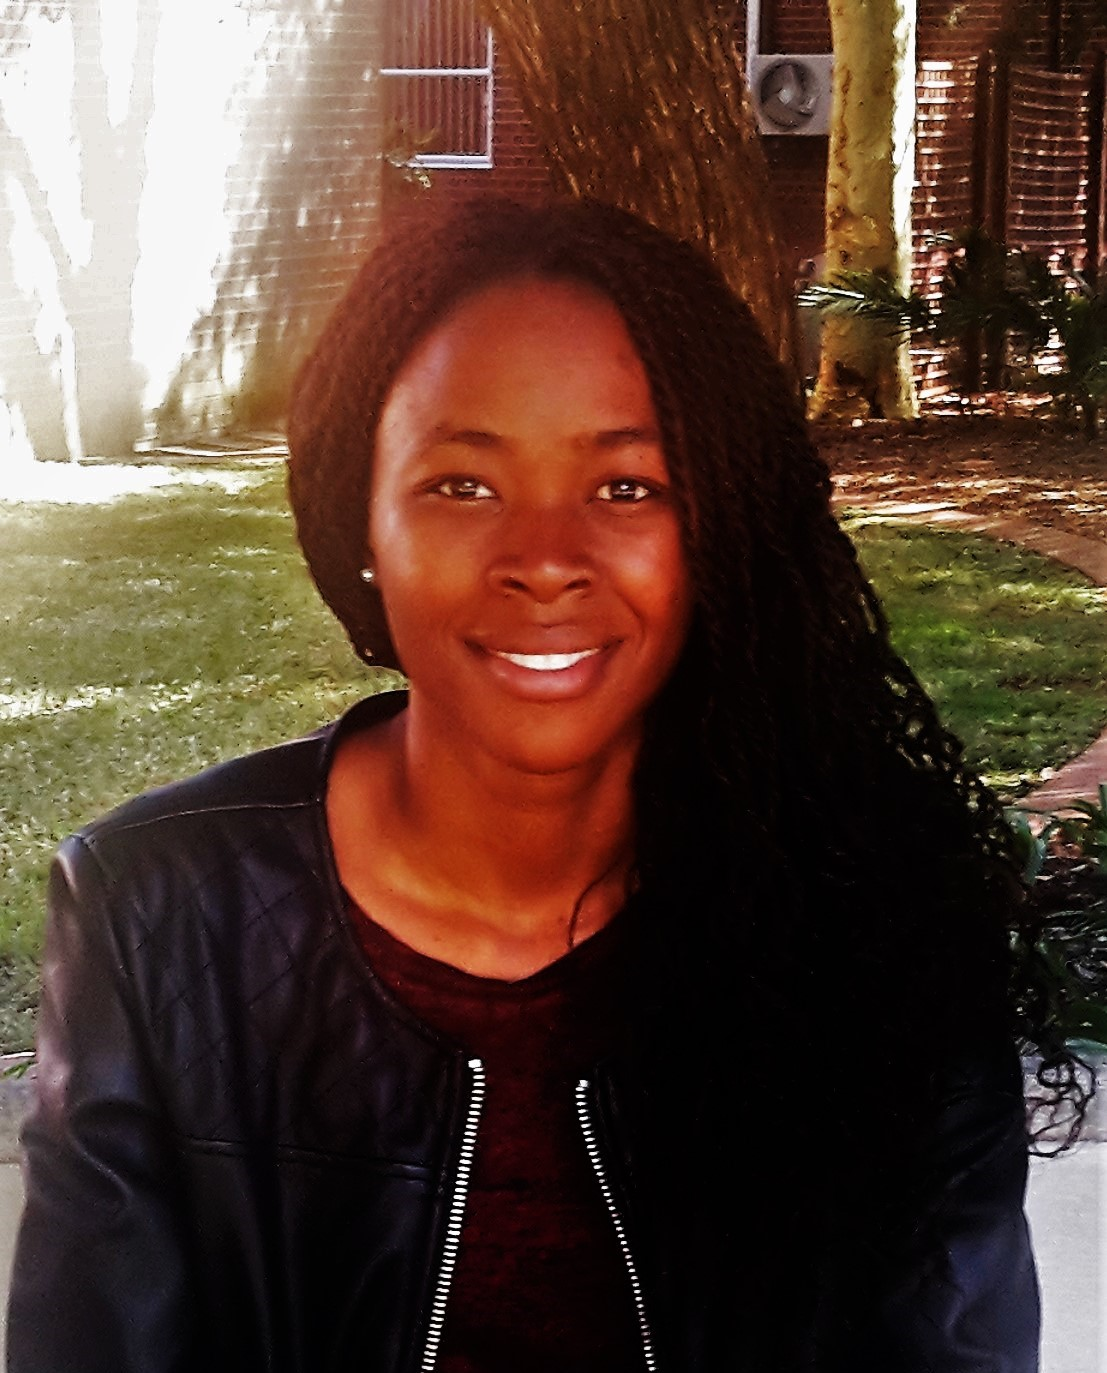
\includegraphics[width= 2in]{Diana.jpg}\\[0.4cm] 
\end{center}

\begin{itemize}
\item {\large \underline{\textbf{Interests}}}\\[0.2cm]
My interests are travelling, game development, Web development and Anime. I also enjoy learning about new technologies and watching a lot of discovery channels and documentaries.

\item {\large \underline{\textbf{Technical Skills}}}
	\begin{itemize}
		\item I have sound knowledge of Java, C++, HTML, CSS, Javascript, C\# and MatLab
		\item Mobile development (Android Studio) 
		\item 3DS MAX.
		\item Ember.js and  Handlebar.js
	\end{itemize}
\bigskip
\item {\large \underline{\textbf{Past Experience}}}
\begin{itemize}
\item I participated in this year's Standard Bank IT Challenge.
\item I did an internship at a small company named Lepsta where I did Web development.
\end{itemize}
\bigskip
\item {\large \underline{\textbf{Non-Technical Skills}}}
\begin{itemize}
\item Willingness to learn
\item Team player
\item Organised
\item Diligent
\item Reliable
\end{itemize}
\bigskip
\item {\large \underline{\textbf{Reason for Interest in the Project}}}\\[0.2cm]
Since I am interested in Game Development, Anime and I’ve worked with 3DS Max, this project will expand my knowledge in Augmented Reality and Computer Graphics.

\end{itemize}
%Diana Obo's Section - end

\newpage

% Kudzai Muranga's Section - start
\begin{center}
{\Large Kudzai {Muranga}} \\[0.3cm]
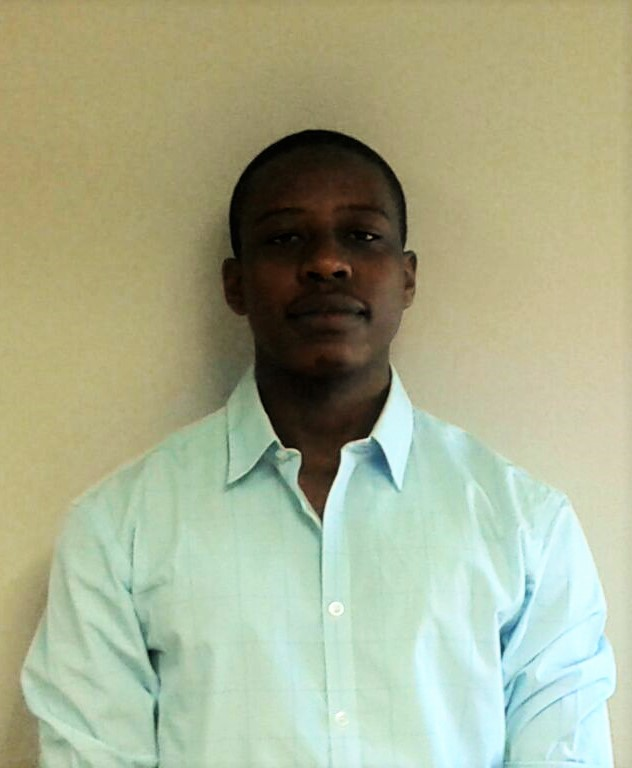
\includegraphics[width= 2in]{Kudzai.jpg}\\[0.4cm] 
\end{center}

\begin{itemize}
\item {\large \underline{\textbf{Interests}}}\\[0.2cm]
I am an avid reader. I love fantasy novels the most. I like to keep myself up to date with the current affairs of the world. I am also interested in learning anything new that concerns science, technology and business.
\\
\item {\large \underline{\textbf{Technical Skills}}}
	\begin{itemize}
		\item I have sound knowledge of Java, C++, HTML, CSS, Javascript, C\# and mobile development 
		\item Artificial Intelligence experience.
		\item Business Management knowledge
		\item Project Management
	\end{itemize}
\bigskip
\item {\large \underline{\textbf{Past Experience}}}
\begin{itemize}
\item I have participated in the Standard Bank IT Challenge.
\item I have been invited to the Hello Group Open Day where I participated in a coding challenge using Java.
\end{itemize}
\bigskip
\item {\large \underline{\textbf{Non-Technical Skills}}}
\begin{itemize}
\item I am interested and open to learning new things
\item Disciplined
\item Organised
\item Critical Thinking
\end{itemize}
\bigskip
\item {\large \underline{\textbf{Reason for Interest in the Project}}}\\[0.2cm]
I am interested in this project because I feel that it would allow me to use programming abilities extensively and teach me new and exciting skills.
% Kudzai Muranga's Section - end

\newpage
%Sandile Khumalo's Section - start
\end{itemize}
\begin{center}
{\Large Sandile {Khumalo}} \\[0.3cm]
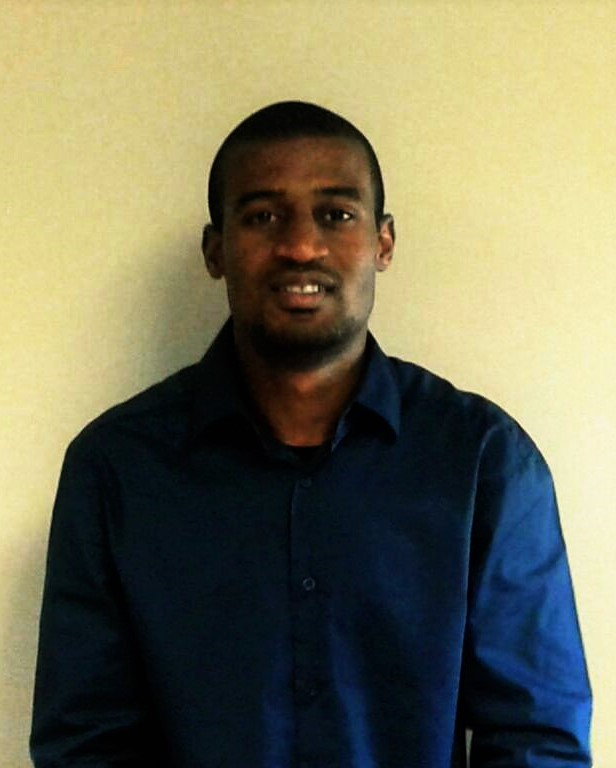
\includegraphics[width=2in]{Sandile.jpg}\\[0.4cm] 
\end{center}



\begin{itemize}
\item {\large \underline{\textbf{Interests}}}\\[0.2cm]
My interest are coding, reading on new and exciting, technologies and watching and reading about football. I also enjoy weightlifting.


\item {\large \underline{\textbf{Technical Skills}}}

	\begin{itemize}
		\item I am comfortable and have experience coding in these languages; C++, Java, C\#, PHP, HTMLl, JavaScript and Bash. I also have done 64 bit assembler language and I have experience in MINIX.
	\end{itemize}
\bigskip
\item {\large \underline{\textbf{Past Experience}}}\\[0.2cm]
I have done a project in my software development class that is similar. It incorporates  most of the technologies and frameworks used in the work place when developing big projects.
\\
\item {\large \underline{\textbf{Non-Technical Skills}}}\\[0.2cm]
 I am a hard working student. I am dedicated and I believe if there is a will, the is a way. This is especially true as a developer because most of the solutions are there and someone has done it before. It's a matter of good research and good understanding of the task at hand. I am willing to learn from every experience. 
\\
\item {\large \underline{\textbf{Reason for Interest in the Project}}}\\[0.2cm]
I find this project challenging and exciting. There is a lot to learn from it. It would be great to work on the Augmented Reality feature and expand my knowledge.

\end{itemize}

%Sandile Khumalo's Section - end
\newpage
%Project Execution
\section{Project Execution}

\begin{itemize}
\item {\large \underline{\textbf{Development Methodology}}}\\[0.2cm]
For this project, the following development methodology will be used:

	\begin{itemize}
 		\item \underline{Name:}
		\\[0.1cm]
		 Scrum
		\item  \underline{What is Scrum?}
		\\[0.1cm]
		Scrum is a lightweight management framework with broad applicability for managing \& controlling iterative \& 				incremental projects of all types (Takeuchi \& Nonaka, 1999).
		\item \underline{Why did we choose to use it?}
		\\[0.1cm]
		Because of all the potential additions that might occur at the different stages of development for this project, we 			have decided that Scrum is the best suited development methodology to use.
	\end{itemize}
\bigskip

\item {\large \underline{\textbf{Keeping the Epi-Use Informed}}}\\[0.2cm]
To keep the client informed about the project, we are going to use the following technologies and strategies:

	\begin{itemize}
	\item During the client meetings where we are going to discuss all aspects of the project.
	\item Send email to set up appointments.
	\item Use an application called Slack for general queries and updates.
	\end{itemize} 

\bigskip
\item {\large \underline{\textbf{Ideas to Solve Technical Problems for VizARD}}}
\begin{itemize}
	\item We will add an API that will help us represent textual data into statistical data.
	\item We will have another API that will help us configure all the different types of graphical representations.
	\item An AI will be devised to automate the creation of 3D models in WebGL. This AI will be optimised for mobile platforms.
	\item A Neural Network will be used to train the AI that will be used to be able to select an appropriate graph for given 			data.
\end{itemize}

\newpage
\item {\large \underline{\textbf{Possible Technologies to be Used}}}\\[0.2cm]
\begin{itemize}
	\item \underline{Character Recognition Library:} Tesseract for mobile platforms
	\\
	\item \underline{Augmented Reality SDK:} Vuforia
	\\
	\item \underline{Unit Testing:}   JUnit Framework
	\\
	\item We will use Maven for dependency management, plugin framework and support for modularization for 				projects.
\end{itemize}


 \item {\large \underline{\textbf{What Epi-Use Labs will Receive}}}\\[0.2cm]
In addition to the project deliverables, the Epi-Use Labs will receive source code that will run on several mobile platforms.
\end{itemize}
\end{document}

